\documentclass[11pt,technote]{IEEEtran}
\usepackage{listings}
\usepackage{graphicx}
\usepackage[noadjust]{cite}
\usepackage{hyperref}
\bibliographystyle{IEEEtran}


\begin{document}
\lstset{language=bash}
%
% paper title
% can use linebreaks \\ within to get better formatting as desired
\title{RSA Cryptosystem Generation of Public and Private Keys in Rust}
\author{~Dr.~Elise~deDoncker,~Jason~Pearson,~Sam~Demorest% <-this % stops a space
\thanks{}}

% The paper headers
\markboth{}%
{Shell \MakeLowercase{\textit{et al.}}: RSA Cryptosystem Generation of Public 
and Private Keys in Rust}



\IEEEcompsoctitleabstractindextext{%
\begin{abstract}
	The goal of our project was to develop two programs. The first program would 
	be for determining large prime numbers and the second program for using the 
	first application to create public and private key pairs and using these pairs 
	to encrypt/decrypt a message.
\end{abstract}
\begin{IEEEkeywords}
RSA, rust, key generation, large prime numbers
\end{IEEEkeywords}}


% make the title area
\maketitle

\IEEEdisplaynotcompsoctitleabstractindextext
\IEEEpeerreviewmaketitle



\section{Introduction}
\IEEEPARstart{T}{his} project under the supervision of Dr. Elise de Doncker is 
to implement the numerous algorithms needed to create a public and private RSA 
key pair set. 


\section{Research}
At the start of our project we first researched what an RSA key is and how to 
generate them and discovered it only takes a few steps. The first step is to 
create two prime numbers. The larger the prime number the better the encryption. 
Then with these two prime numbers we would be able to create a public and 
private key \cite{fastrsa}. 

\par We found two algorithms for finding if a number is prime or 
not. The first is the AKS Primality Test. This primality test is the best 
deterministic primality test known in terms of time complexity \cite{neap}.
This being said it is still very slow when compared to non deterministic 
primality testing algorithms. So we also looked at the Miller Rabin 
probabilistic primality tests to also test numbers which runs much faster than 
the AKS primality test. In the end, and explained later, we chose the 
Miller-Rabin test, in part because of performance, and in part because the 
language we were using has not yet implemented any logarithm operations for its 
BigInt types.

\section{Design}
First we needed to select a programming language. We both had expressed 
interest in the new beta programming language Rust and after some research we 
discovered that it would be a good language to use. Rust is an open-source 
compiled language that is syntactically similar to C and C++ with an emphasis on 
control of memory layout and safety.  

\par After choosing what language we were going to use the first thing we did 
was see if someone had already created a primality testing library that we could 
use. Upon inspecting the algorithms that were available in the libraries on 
crates.io used the Sieve of Eratosthenes technique. This algorithm calculates 
all numbers that are less than n that are prime. This is good for if you need 
small prime numbers, but our goal was to generate large prime numbers. 

\par With no library available we decided that we would have to create our own 
large prime generator. Because there was no library available we decided to pull 
that section of code out and create our own library. Once the project is 
completed that section of code will be publicly available on GitHub under 
MIT/Apache-2.0 license.


\section{Implementation}
The prime generator used the Miller-Rabin testing for our generation of prime
numbers, for reasons discussed below. Before any test was used we made sure the
number wasn't even to make sure we aren't using lots of time for easy to find 
compound numbers.
\par Here we have a slight discrepancy between the initial design proposal and
our finished product. In the design document our group submitted, we said we
would be using the AKS deterministic polynomial-time test for primality.
Unfortunately, this was not possible using Rust. For encryption keys, we want
arbitrarily large numbers, which requires the use of a BigInt type.
However, there are no logarithm operations supported on this data type,
and logarithms are essential to the calculations involved in the AKS test for
primality. Rather than expend effort contributing code to the core of the
language we chose to use so that we could implement this primality test, we
decided instead that the Miller-Rabin probabilistic test for primality would
meet our needs for the purposes of this project. Had we chosen a different, more
mature language at the start of our project, we would have been able to
implement the AKS test. However, by the time we realized that implementing this
test would be impossible in the language that we chose, we had already
implemented too much of the rest of the program for us to discard what we had
accomplished.
\par The key generator calls the prime generation method of the first program 
and that takes care of all the work for prime number generation. After it gets 
the prime numbers p and q we use those to compute n which is simply p times q. 
Next we determine φ(n) which is simply $n - (p + q -1)$. After these are all 
computed we create a good e value and compute d. The e value is simply a number 
\\1 $<$ e $<φ(n)$. Then d = e$^{-1}$(mod(φ(n)), which is the private key part of 
the encryption.


\section{Testing}
Since the two programs were separate we had a rather easy time testing each one 
out individually. 
For our prime number generator it was fairly simple to determine that our test 
is working correctly. All that we had to do was send in some numbers that we 
know are prime and some that are not prime and make sure that the test
responded accordingly.
\par To test our program we took an example and tested that our input and output 
matched. For the example we took some small prime numbers just for testing. So 
for p and q we took the values 61 and 53 respectively. Then we know that it 
should calculate for n as 3233 and we know that the totient that it creates 
should be 3120. For e we need to assign it a value so we can calculate the other 
values correctly. So for this example we chose 17 and when we calculate the d 
value we get 2753. 
\par Now using those values we can compute what A should encrypt to and 
determine if our program is encrypting the value correctly. So the ASCII value 
of A is 65, so our ciphertext would be ${65}^{17}\mathrm{mod}3233=2790$. So for 
our test values we know that A should be encrypted to 2790. For testing our 
decryption part we just have to make sure it calculates 2790 back to A.

\subsection{Performance Measurements}
\par As we were implementing this program, it became clear that modulo
exponentiation was the bottleneck in the performance of our program. Modulo
exponentiation is used in the process of generating prime numbers, as well as in
the processes of encryption and decryption. With such a ubiquitous algorithm, it
was important that we had an efficient algorithm. We began with a naive
implementation of modulo exponentiation, and we also implemented an optimized
algorithm documented by Bruce Schneier \cite{sonsec}.
\begin{figure}
	\begin{center}
		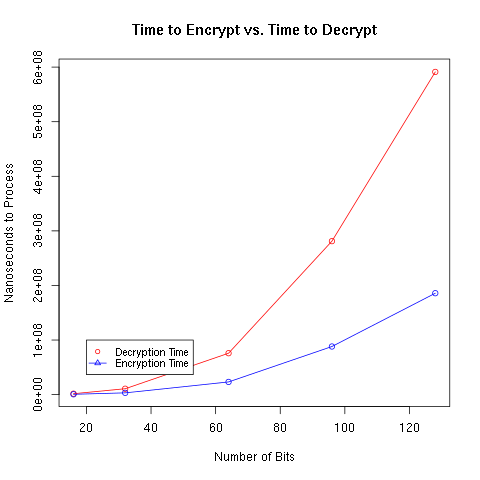
\includegraphics[width=0.5\textwidth]{cryptimes}
		\caption{Increasing time with increasing bit-size of keys}
	\end{center}
\end{figure}
\par It is clear to see that encryption and decryption both follow polynomial
curves as the number of bits used in the encryption process increase, with
decryption increasing at a much faster rate than decryption. This is exhibited
in Figure 1.
\begin{figure}
	\begin{center}
		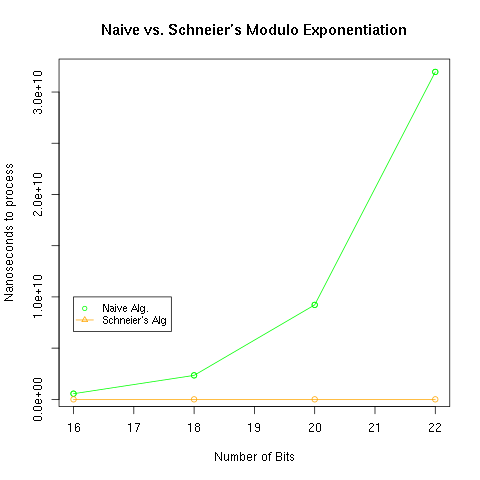
\includegraphics[width=0.5\textwidth]{modexp}
		\caption{Time complexity between a naive implementation of modulo
		exponentiation and Schneier's modulo exponentiation\cite{sonsec}}
	\end{center}
\end{figure}
\par There is a substantial difference in the rates of growth in reference to
the time these two algorithms take. The naive algorithm grows exponentially, as
it is an exponentiation function. While the complexity scales linearly with the
power to which a number is being brought, in the context of input size, that is 
the number of bits in the power, the rate of growth is approximately $2^s$
\begin{figure}
	\begin{center}
		\lstinputlisting[basicstyle=\tiny,firstline=78,lastline=97]{prime.rs}
		\caption{Schneier's Modulo Exponentiation Implemented in Rust\cite{sonsec}}
	\end{center}
\end{figure}
\par We can see in this code that the time complexity of this algorithm is going
to be linear in relation to the input size $s$, which is defined as the number
of bits required to represent the power to which the base is being brought. Each
iteration through the loop, the power is bit-shifted to the right by one bit,
until eventually the power reaches zero. This complexity for the algorithm
should be immediately apparent when studying the code in Figure 3, and studying
the chart in Figure 2 will provide a clue that this algorithm is likely linear
in time complexity.
\par We were able to generate the data used for this analysis using the Rust
language's built in testing suite. We made extensive use of Rust's testing
capabilities, following a test-drived development lifecycle, and using tests to
verify the correctness of the algorithms being implemented. The actual analysis
of the data was conducted using the R programming language, which is
particularly well-suited for this type of analysis.
\section{Goals Reached}
Our initial goals were to create a primality testing section and to create 
public and private keys. We were successful in testing for prime numbers with a 
a non-deterministic method. Another goal of ours was to encrypt and decrypt an 
input string and we were also successful in this goal. Using the fast modulo
exponentiation shown in Figure 3, we were able to use keys of up to 224 bits in
a practical amount of time.
\par One of our stretch goals was not reached. We were hoping to be able to use 
our program with other programs that use public and private key pairs such as 
ssh. We determined this to be out of scope because of the strict standards set 
up by the IEEE. 

\section{User Guide}
To run this program it is very simple. First you will need to build the program 
so cd to the directory and run 
\begin{lstlisting}[basicstyle=\small]
cargo build
\end{lstlisting} 
This compiles the program then to run it we simply do 
\begin{lstlisting}[basicstyle=\small]
cargo run X 
\end{lstlisting}
Where X is the bit size. The larger the bit size the longer the program will 
run. After you run the application it will ask for a character you would like 
encrypted then decrypted. Figure 4 exhibits an example run of the program.
\begin{figure}
	\begin{center}
		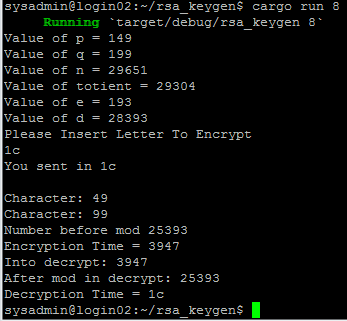
\includegraphics[width=0.5\textwidth]{Capture.PNG}
		\caption{Screenshot of the RSA program output}
	\end{center}
\end{figure}

\section{Conclusion}
The program does generate large prime numbers as it is advertised to do, however 
with the larger bit sizes the time to calculate a prime number takes a very long 
time. Keeping in mind that finding a prime number is polynomial in terms of 
complexity it should be understood that there is no better way to do this. This 
program is capable of encrypting using arbitrary key sizes, but the performance
of Rust's arbitrarily sized integers is still lacking, so performance degrades
quickly the larger the key size gets. Additionally, we focused on code
readability and reusability, and so did not implement any particularly
sophisticated optimizations in our encryption program. As a result, we are only
able to use keys up to 224 bits in a practical amount of time. This is greatly
already greatly improved by Schneier's modulo exponentiation algorithm, and is a
better result than we had anticipated. However the language is still in its beta 
phases so as it becomes more developed there will be more support for complex 
computations. Even with these challenges we were able to create a program that 
met most of our goals and was able to actually encrypt and decrypt information 
so we think that the project was successful.
\cite{sonsec}

\bibliography{biblio}
\end{document}


